%% Source of figures/benchmark-pipeline.pdf (rules/04-figures-tables.md).
%% Build: xelatex -output-directory=figures figures/src/benchmark-pipeline.tex
%% Drawn from opentrading-benchmark 3be3e1b (finance-v47-study: run_benchmark.py, judge_primary.py,
%% runners/, runners/sandbox), the sealed configuration of run main-20261124 and the amendment of 25/11/2026.
\documentclass[border=2pt]{standalone}
\usepackage{fontspec}
\IfFontExistsTF{Arial}{\setmainfont{Arial}}{\setmainfont{TeX Gyre Heros}}
\usepackage{tikz}
\usetikzlibrary{positioning,arrows.meta,fit,backgrounds}
\begin{document}
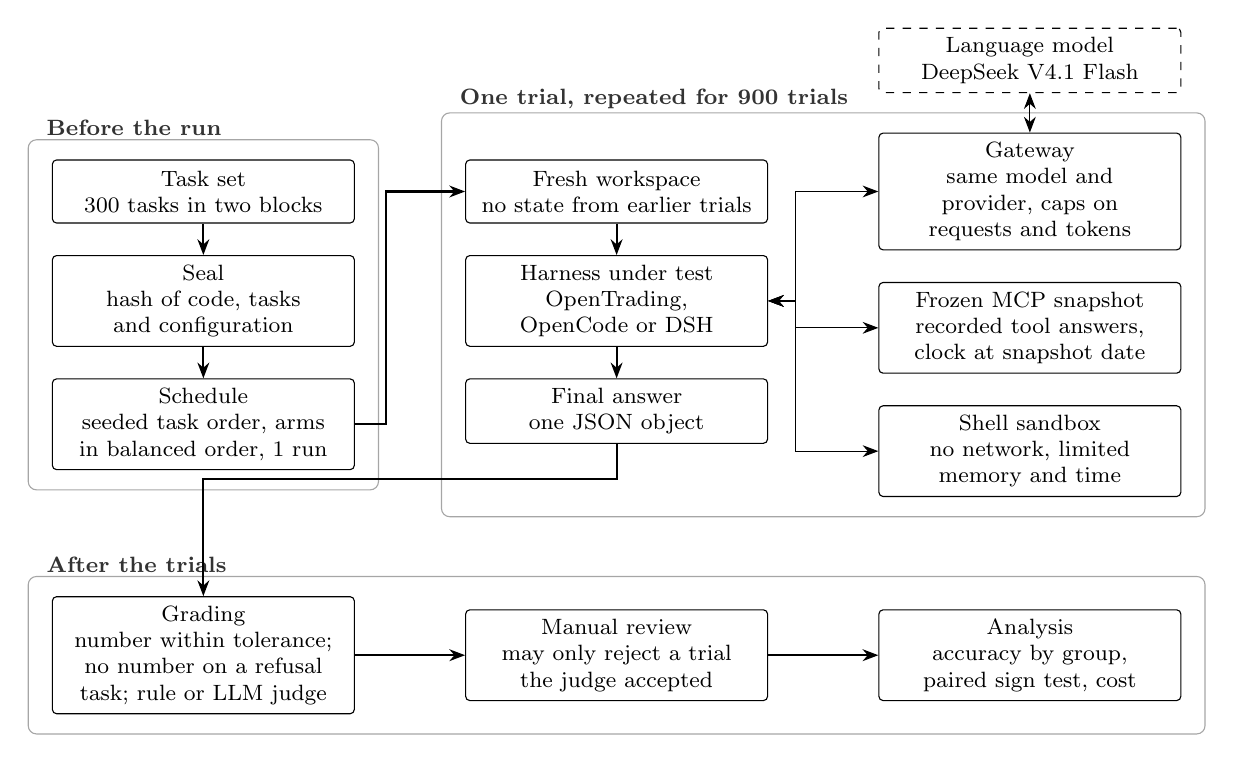
\begin{tikzpicture}[
  font=\fontsize{8}{9.5}\selectfont,
  node distance=4mm and 7mm,
  box/.style={draw, rounded corners=1.5pt, align=center, text width=36mm, minimum height=8mm, fill=white, execute at begin node={\hyphenpenalty=10000\relax}},
  ext/.style={box, dashed},
  arr/.style={-{Stealth[length=2mm]}, thick},
  two/.style={{Stealth[length=2mm]}-{Stealth[length=2mm]}},
  group/.style={draw, gray!70, rounded corners=3pt, inner xsep=3mm, inner ysep=2.5mm},
  glabel/.style={font=\fontsize{8}{9.5}\selectfont\bfseries, anchor=south west, gray!40!black, inner sep=1pt}
]
% Column 1: preparation
\node[box] (tasks) {Task set\\300 tasks in two blocks};
\node[box, below=of tasks] (seal) {Seal\\hash of code, tasks and configuration};
\node[box, below=of seal] (sched) {Schedule\\seeded task order, arms in balanced order, 1 run};

% Column 2: one trial
\node[box, right=14mm of tasks] (ws) {Fresh workspace\\no state from earlier trials};
\node[box, below=of ws] (arm) {Harness under test\\OpenTrading, OpenCode or DSH};
\node[box, below=of arm] (ans) {Final answer\\one JSON object};

% Column 3: shared environment
\node[box, right=14mm of ws] (gw) {Gateway\\same model and provider, caps on requests and tokens};
\node[box, below=of gw] (mcp) {Frozen MCP snapshot\\recorded tool answers, clock at snapshot date};
\node[box, below=of mcp] (sbx) {Shell sandbox\\no network, limited memory and time};
\node[ext, above=5mm of gw] (llm) {Language model\\DeepSeek V4.1 Flash};

% Row below: grading and analysis
\node[box, below=16mm of sched] (grade) {Grading\\number within tolerance; no number on a refusal task; rule or LLM judge};
\node[box, right=14mm of grade] (rev) {Manual review\\may only reject a trial the judge accepted};
\node[box, right=14mm of rev] (ana) {Analysis\\accuracy by group, paired sign test, cost};

\draw[arr] (tasks) -- (seal);
\draw[arr] (seal) -- (sched);
\draw[arr] (sched.east) -- ++(4mm,0) |- (ws.west);
\draw[arr] (ws) -- (arm);
\draw[arr] (arm) -- (ans);
\draw[two] (arm.east) -- ++(3.5mm,0) |- (gw.west);
\draw[two] (arm.east) -- ++(3.5mm,0) |- (mcp.west);
\draw[two] (arm.east) -- ++(3.5mm,0) |- (sbx.west);
\draw[two] (gw) -- (llm);
\draw[arr] (ans.south) -- ++(0,-4.5mm) -| (grade.north);
\draw[arr] (grade) -- (rev);
\draw[arr] (rev) -- (ana);

\begin{scope}[on background layer]
  \node[group, fit=(tasks)(sched)] (prep) {};
  \node[glabel] at ([xshift=2mm]prep.north west) {Before the run};
  \node[group, fit=(ws)(ans)(gw)(sbx)] (trial) {};
  \node[glabel] at ([xshift=2mm]trial.north west) {One trial, repeated for 900 trials};
  \node[group, fit=(grade)(ana)] (after) {};
  \node[glabel] at ([xshift=2mm]after.north west) {After the trials};
\end{scope}
\end{tikzpicture}
\end{document}
